\documentclass[a4paper]{sbgames}               % final
%\usepackage[scaled=.92]{helvet}
\usepackage[utf8]{inputenc}
%\usepackage[brazil]{babel}
%\usepackage[latin1]{inputenc}
\usepackage{times}
\usepackage{graphicx}

%% use this for zero \parindent and non-zero \parskip, intelligently.
\usepackage{parskip}

%% the 'caption' package provides a nicer-looking replacement
\usepackage[labelfont=bf,textfont=it]{caption}

\usepackage{url}



\usepackage{array}
\usepackage[dvips]{color}
%\usepackage{fancyvrb,moreverb}
\usepackage{listings}
\usepackage{units}

\definecolor{gray}{rgb}{.9,.9,.9}




%% Paper title.
\title{FPS: First ``Paper''  Shooting}

%% Author and Affiliation (multiple authors). Use: and between authors

\author{Name1 A. Surname1\\ Digital Games Lab 
        \and Name2 B. Surname2\\ Name3 C. Surname3\\ ZZZZ University
        \and Name4 D. Surname4\\ Farwest Research Center 
}
\contactinfo{\{name1,name3\}@xxx.yyyy.yyy \\
             *name2@zzzz.vvvv.vvv
}
%% Keywords that describe your work.
\keywords{Real-time Strategy, Relief Mapping, Shortest Path Algorithm, First Person Shooting}

%% Start of the paper
% Attention: As you need to insert EPS images in Postscript, 
% you need to insert PDF images into PDFs. 
% In the text, extensions cancbe omitted (latex use .eps, pdflatex get .pdf) 
% To convert them: epstopdf myimage.eps
\begin{document}

%\teaser{
%  \includegraphics[width=\linewidth]{sample.pdf}
%  \caption{Optional image}
%}

%% The ``\maketitle'' command must be the first command after the
%% ``\begin{document}'' command. It prepares and prints the title block.

\maketitle

%% Abstract section.

\begin{abstract}
  O protocolo UPnP visa prover uma forma de conexão simples, robusta e interativa entre dispositivos móveis, eletroeletrônicos e até eletrodomésticos provenientes de diversos fabricantes. Apesar de um padrão internacional emergente(2008), tem se tornado bastante popular na indústria por tais características permitindo novas funcionalidades com o desenvolvimento de diversas aplicações, por conseguinte, introduzindo a nova era de computação pervasiva. Devido a pervasividade do UPnP, que utiliza um sistema eficaz de descoberta de dispositivos, torna-se possível a integração instantânea de novos dispositivos em uma rede local. Assim, tal protocolo pode ser usado para implementar um ambiente pervasivo para jogos eletrônicos. Portanto, este trabalho apresenta uma nova utilidade para o protocolo UPnP: prover serviços e funcionalidades para jogos eletrônicos, introduzindo um servidor de jogos pervasivo: o BRiGaS(BRrisa Game Server), que extende o framework BRisa para o protocolo UPnP, adicionando funcionalidades para ambientes de jogos. A pervasividade provida e a possibilidade do uso de jogos portáveis facilita e torna mais divertida a integração e interação entre jogadores.
\end{abstract}

%% The ``\keywordlist'' command prints out the keywords.
\keywordlist
\contactlist

\section{Introdução}

<<<<<<< TREE
Devido a explosão e popularização do consumo de dispositivos móveis e a initerrupta evolução da tecnologia móvel, novos conceitos de tecnologia surgem. A pervasividade permite que dispositivos entrem em uma rede local automaticamente interagindo e fazendo uso de serviços providos por elementos do domínio da rede, em seu estado da arte estaria em todos os lugares, em vários ambientes, o dispositivo se comunicaria com várias redes de forma transparente e interativa. O padrão UPnP vem sendo amplamente utilizado para flexibilizar e facilitar a integração de dispositivos em uma rede local. Pela fácil implantação e seu sistema de descoberta de dispositivos ser eficaz, somados à utilização de tecnologias abertas consagradas da internet como HTTP, XML e SOAP, este padrão é uma forte escolha para criar sistemas pervasivos. 

Devido as suas características, é util criar um servidor de jogos usando a tecnologia UPnP especificando um dispositivo UPnP centrados em jogos, definindo dessa forma um servidor de jogos interoperável, aceitando clientes de diversas naturezas como celulares, PDAs, internet tablets, computadores desktop, consoles de vídeo games e qualquer outro dispositivo eletrônico capaz de implementar o padrão. Nesse cenário as pessoas podem jogar em rede através de seus dispositivos, interagindo com o(s) servidor(es) de jogos disponíveis no ambiente sem a necessidade de configurar diretamente seus dispositivos.

Porém, o uso do padrão UPnP no universo dos jogos eletrônicos se dá atualmente ao uso de media servers, controle remoto e mecanismos para facilitar o acesso às redes locais.  Portanto, este trabalho introduz uma nova possibilidade ao uso do padrão UPnP: prover controle e interação para jogos eletrônicos através de serviços providos por um dispositivo centrado em jogos. Foi então especificado um padrão para servidores de jogos UPnP e também foi feita a implementação da mesma, de código aberto e portável que permita a interação entre diversos dispositivos, o BRiGaS(BRisa Game Server).

O BRiGas(BRisa Game Server) está sendo desenvolvido utilizando o framework para UPnP BRisa, desenvolvido pelo Embedded Lab de Campina Grande. A implementação do Game Server já incitou em questionamentos e alterações na implementação do framework, influenciando e contribuíndo em seu desenvolvimento. Também, levanta algumas questões sobre o funcionamento do padrão UPnP para o uso em certas aplicações em que os dispositivos de uma rede local interajam de forma similar a jogos eletrônicos. Também foi implementado um jogo de cartas como caso de teste para o servidor de jogos.

O trabalho será detalhado nas próximas sessões como segue: depois de apresentar algumas características do padrão UPnP na seção 2, serão abordados alguns cenários do funcionamento do Game Server utilzando o UPnP na seção 3. Também, na seção 4 será apresentada a especificação do Game Server seguida pela apresentação de sua implementação na seção 5. Em seguida, será apresentado um teste de conceito na seção 6, juntamente com as conclusões do trabalho na seção 7.

=======
Devido a explosão e popularização do consumo de dispositivos móveis e a initerrupta evolução da tecnologia móvel, novos conceitos de tecnologia surgem. A pervasividade permite que dispositivos entrem em uma rede local automaticamente interagindo e fazendo uso de serviços providos por elementos do domínio da rede, em seu estado da arte estaria em todos os lugares, em vários ambientes, o dispositivo se comunicaria com várias redes de forma transparente e interativa. O padrão UPnP vem sendo amplamente utilizado para flexibilizar e facilitar a integração de dispositivos em uma rede local. Pela fácil implantação e seu sistema de descoberta de dispositivos ser eficaz, somados à utilização de tecnologias abertas consagradas da internet como HTTP, XML e SOAP, este padrão é uma forte escolha para criar sistemas pervasivos.

Devido as suas características, é útil criar um servidor de jogos usando a tecnologia UPnP especificando um dispositivo UPnP centrados em jogos, definindo dessa forma um servidor de jogos interoperável, aceitando clientes de diversas naturezas como celulares, PDAs, internet tablets, computadores desktop, consoles de vídeo games e qualquer outro dispositivo eletrônico capaz de implementar o padrão, como exemplificado na figura1. Nesse cenário as pessoas podem jogar em rede através de seus dispositivos, interagindo com o(s) servidor(es) de jogos disponíveis no ambiente sem a necessidade de configurar diretamente seus dispositivos.

\begin{figure}[h!]
    \centering
    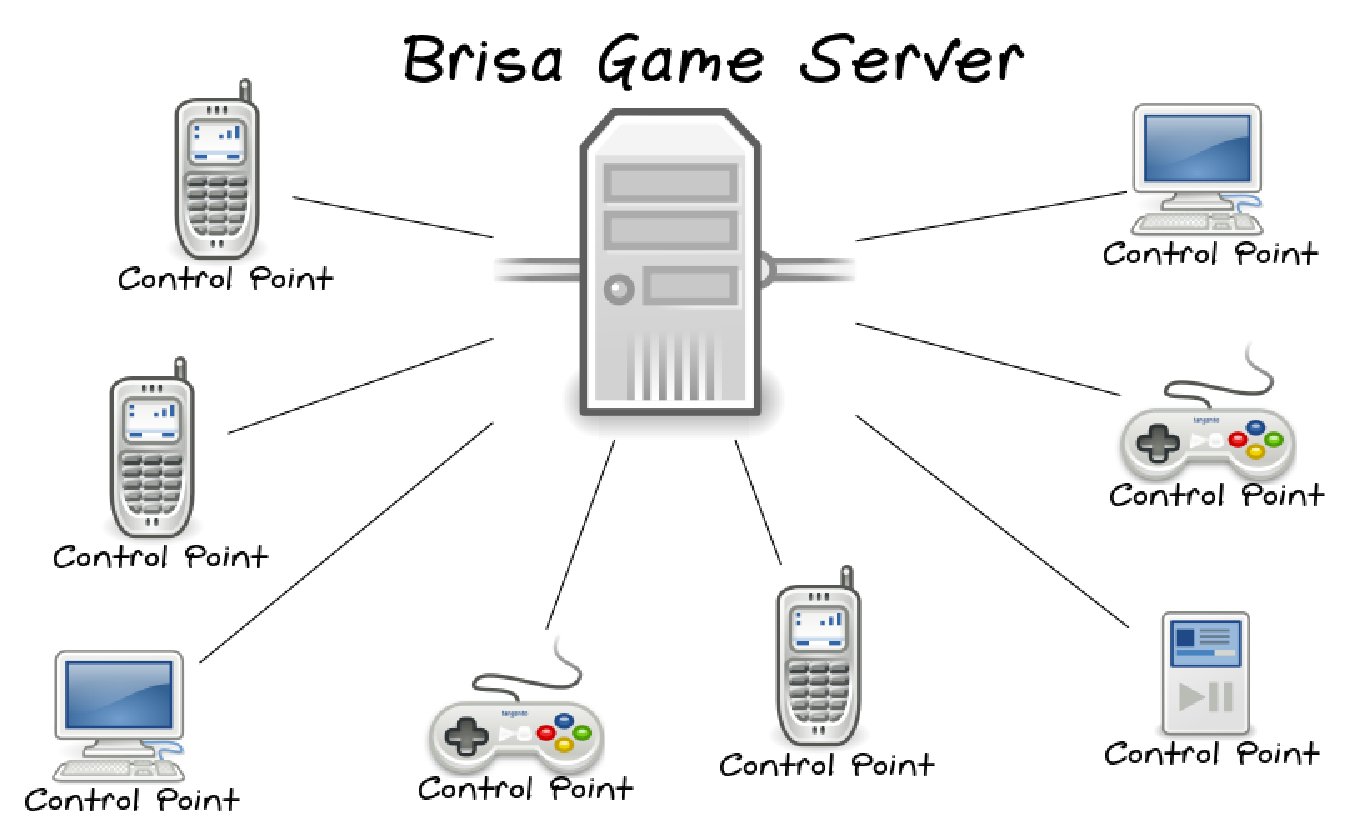
\includegraphics[scale=0.35]{images/brisa-game-server.eps}
    \caption{Esquema do funcionamento do BRisa Game Server(BRiGaS).}
    \label{fig:avschema_new}
\vspace{-5mm}
\end{figure}
\vspace{3mm}
\normalsize

Porém, o uso do padrão UPnP no universo dos jogos eletrônicos se dá atualmente ao uso de media servers e renderers, controle remoto e mecanismos para facilitar o acesso às redes locais.  Portanto, este trabalho introduz uma nova possibilidade ao uso do padrão UPnP: prover controle e interação para jogos eletrônicos através de serviços providos por um dispositivo centrado em jogos. Foi então especificado um padrão para servidores de jogos UPnP e também foi feita a implementação da mesma, de código aberto e portável que permita a interação entre diversos 
dispositivos, o BRiGaS (BRisa Game Server).

O BRiGaS (BRisa Game Server) está sendo desenvolvido utilizando o framework para UPnP BRisa, desenvolvido pelo Embedded Lab de Campina Grande. A implementação do Game Server já incitou em questionamentos e alterações na implementação do framework, influenciando e contribuíndo em seu desenvolvimento. Também levanta algumas questões sobre o funcionamento do padrão UPnP para o uso em certas aplicações em que os dispositivos de uma rede local interajam de forma similar a jogos eletrônicos. Foi implementado um jogo de cartas como caso de teste para o servidor de jogos.

O trabalho será detalhado nas próximas sessões como segue: depois de apresentar algumas características do padrão UPnP na seção 2, serão abordados alguns cenários do funcionamento do Game Server utilzando o UPnP na seção 3. Também, na seção 4 será apresentada a especificação do Game Server seguida pela apresentação de sua implementação na seção 5. Em seguida, será apresentado um teste de conceito na seção 6, juntamente com as conclusões do trabalho na seção 7.

>>>>>>> MERGE-SOURCE

\section{Overview and background}
\subsection{UPnP Overview}
<<<<<<< TREE
UPnP é uma tecnologia de padrão internacional cuja especificação foi divulgada no meio de 2002 pelo UPnP Forum[4].Carrega consigo uma descoberta de dispositivos e invocação de serviços baseado em tecnologias da Internet como HTTP, XML e SOAP,  divididos em seis passos: endereçamento, descoberta, descrição, controle, geração de eventos e apresentação. O protocolo UPnP primeiro usa o ponto de controle [6], como primeiro passo para descobrir dispositivos habilitados a utilizar o UPnP, que podem ser filtrados de acordo com a preferência do usuário ou do tipo de dispositivo desejado. O processo de descoberta, permite descrição, onde o control point aprende sobre as capacidades dos dispositivos. Para enviar comandos aos dispositivos designados, o control point utiliza o step of control. No passo de geração de eventos, o control point continua escutando as mudanças de estado nos dispositivos, atualizando a interface gráfica do usuário adequadamente, que está definida no passo de apresentação. Já no processo de descoberta, o control point envia uma mensagem multicast do tipo M-SEARCH [6], para descobrir quais dispositivos UPnP estão on-line. Os dispositivos remotos que rodam o protocolo de descoberta UPnP anunciam o estado deles, mandando de volta uma mensagem NOTIFY unicast ao control point. Um exemplo desta mensagem é mostrado no Listening 1. Nesta mensagem, o dispositivo especifica as informaçôes essenciais e um ponteiro - uma URL para um arquivo XML - que permite ao control point proceder com os próximos passos do UPnP descritos acima.

<<exemplo do artigo do Sales>>

Através da URL listada no campo LOCATION (linha 4), o control point descobre mais informações sobre os dispositivos e ponteiros para invocação de serviços por SOAP. A URL de descrição do dispositivo aponta para uma instância XML cujos XML default schema definem propriedades, tais como nome do dispositivo, versão e modelo, URL's para o diretório de serviços dos dispositivos, URL's para registrar eventos de dispositivo, entre outras informações úteis. Um dos exemplos mais populares que ajuda a entender um dispositivo UPnP é a interação entre dispositivos UPnP A/V [11], mostrado na Figura 1. Este é um esquema de como um control point procura objetos multimídia a partir de um media server e os renderiza dentro do media renderer.

Figure 1. A/V UPnP devices communication.

Basicamente, há três entidades principais na especificação UPnP A/V: o Media Server, o Media Render e o Control Point. O media server é responsável por compartilhar objetos multimídia UPnP [6], como áudio, vídeo, arquivos de imagem, rádios da Internet e álbuns de fotografia on-line. Então, estes objetos multimídias podem ser armazenados no sistema de arquivos local, nos hosts da rede local ou mesmo remotamente na Internet. De modo semelhante, o media render é capaz de reproduzir todos os dados multimídias compartilhados por qualquer UPnP media server. Quando um control point é iniciado, ele envia a mensagem de descoberta (passo 1 da Figura 1) para procurar todos os UPnP media servers e media renderers. Cada um dos servidores disponíveis na rede responde à solicitação dos control points que, a partir deste momento, passa a conhecer. Como resultado, um usuário que roda o control point no dispositivo dele pode renderizar qualquer objeto multimídia compartilhado por um media server simplesmente procurando um media server específico.
=======

De acordo com Thiago B. M. de Sales[X], o UPnP é uma especificação que junta a descoberta de dispositivos com a utilização de serviços utilizando tecnologias consagradas da internet, como HTTP, XML e SOAP. A sua funcionalidade é descrita por seis passos: \emph{endereçamento}, \emph{descoberta}, \emph{descrição}, \emph{controle}, \emph{eventos} e \emph{apresentação}.

Considerando que o \emph{endereçamento} IP dos control points e devices está devidamente correto, então a \emph{descoberta} dos devices é feita. Durante o processo de \emph{descoberta}, a \emph{descrição} do device é enviada, e o control point descobre suas as informações. Os control points podem fazer o \emph{controle} dos devices enviando comandos aos mesmos. Utiliza-se de \emph{eventos} para os devices se comunicarem com os control points, onde estes esperam acontecer algo no device para que os informe através de \emph{eventos}. Finalmente após enviar e receber informações, o control point pode utilizar da \emph{apresentação} para as atualizar da forma desejada.
>>>>>>> MERGE-SOURCE

<<<<<<< TREE
No caso do BRiGaS, um UPnP Control Point descobre um Game Server Device(UPnP) na rede, ao identifcar seu tipo, o control point já pode conversar com o serviço Game Manager, este último é encarregado de gerenciar os jogadores e as salas de jogos. Cada jogo neste servidor possui salas, que são criadas pelos próprios jogadores. As salas são ambientes virtuais onde os jogadores se encontram para começar uma partida. Então os control points se comunicam com o Game Manager para saber sobre salas existentes, criar novas e se juntarem às salas existentes. Ao começar uma partida o Game Manager libera o controle da partida para o serviço do jogo em questão. A figura X exemplifica melhor essa questão.
<<Figura do Punk>>
=======
No caso do BRiGaS(figura 1), um UPnP Control Point descobre um Game Server Device(UPnP) na rede, ao identifcar seu tipo, o control point já pode conversar com o serviço Game Manager, este último é encarregado de gerenciar os jogadores e as salas de jogos. Cada jogo neste servidor possui salas, que são criadas pelos próprios jogadores. As salas são ambientes virtuais onde os jogadores se encontram para começar uma partida. Então os control points se comunicam com o Game Manager para saber sobre salas existentes, criar novas e se juntarem às salas existentes. Ao começar uma partida o Game Manager libera o controle da partida para o serviço do jogo em questão.

\begin{figure}[h!]
    \centering
    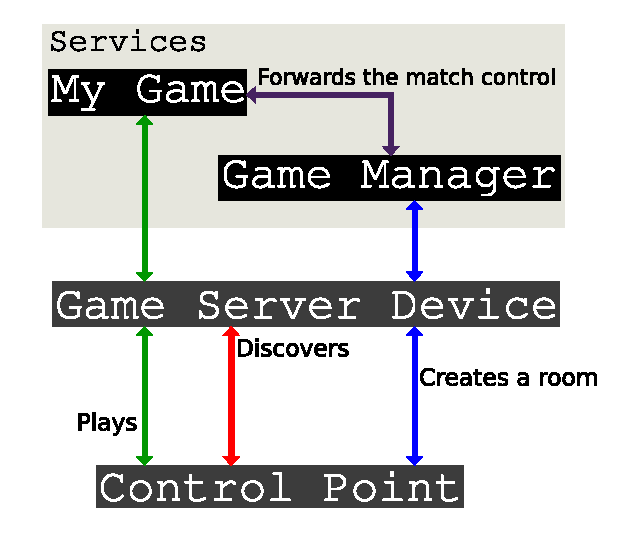
\includegraphics[scale=0.80]{images/game-server-fluxo.eps}
    \caption{Esquema do funcionamento do BRisa Game Server(BRiGaS).}
    \label{fig:avschema_new}
\vspace{-5mm}
\end{figure}
\vspace{3mm}
\normalsize
>>>>>>> MERGE-SOURCE

\subsection{BRisa Framework}

BRisa é um framework que utiliza a tecnologia UPnP. Implementa a arquitetura UPnP escrita na linguagem de programação Python. Inicialmente, foi utilizada uma abordagem que adotou a parte de áudio/vídeo do UPnP como foco principal. Atualmente, alcançou-se um estado de framework geral para UPnP. Além disso, possui certas características como: API de alto nível para construir dispositivos UPnP e serviços através da utilização de programação orientada a objeto, integração com Qt, Gtk, Glib2 e Ecore, implementa facilidades para login, configuração, multi-threading, networking e possui ferramentas para trabalhar com UDP, HTTP, XML, IP e interfaces de rede.

\section{Especificação do Game Server}
O Game Server controla e possibilita a interação de dispositivos durante uma sessão
O Game Server posssibilita a interação de vários dispositivos para um objetivo comum, jogar um determinado jogo entre si.
Essa especificação se divide em duas partes: O Game Server Device, o dispositivo propriamente dito, e o serviço Game Manager, encarregado de gerenciar os jogos e os jogadores do servidor.
\subsection{Game Server Device}
<<<<<<< TREE
No contexto de um servidor de jogos, este deve disponibilizar pelo menos um jogo para que as pessoas possam jogar, e também deve gerenciar como estas pessoas possam reconhecer esses jogos. 
Abstraindo essa questão para o UPnP foi criada a seguinte temática: Existe um dispositvo UPnP, denominado Game Server, e cada jogo dentro deste servidor é um serviço UPnP provido pelo mesmo. Isto quer dizer que para cada jogo existente no servidor, existe um serviço relacionado, que é através dele que os control points se comunicarão para assim serem feitas as jogadas pelos clientes. Estes serviços de jogos não são descritos por essa especificação do Game Server, pois cada jogo tem a sua forma de comunicação e não há como criar uma comunicação padrão para todos os tipos de jogos existentes. Mas um único ponto é requerido para estes serviços de jogos, que de alguma forma eles devem possuir os UUIDs dos jogadores que estão em partida ativa neste jogo, isso será descrito detalhamente mais adiante na seção 3.2. Como este servidor deve gerenciar os jogadores e o acesso dos mesmos aos jogos, foi criado o serviço UPnP Game Manager, que faz parte deste dispositivo, que é encarregado de gerenciar todos os jogadores conectados ao servidor, bem como quais jogos estão disponíveis e também e a transição dos jogodores entre os jogos e suas salas, mais detalhes estão na seção 3.2.
Sendo assim, um Game Server Device deve possuir a seguinte especificação XML:
=======
No contexto de um servidor de jogos, este deve disponibilizar, ao menos, um jogo e também deve gerenciar como os jogadores podem reconhecer esses jogos.
Tornando abstrato este fato para o UPnP, foi criada a seguinte temática: Existe um dispositvo UPnP, denominado Game Server, e cada jogo dentro deste servidor é um serviço UPnP provido pelo mesmo. Isto quer dizer que para cada jogo existente no servidor, existe um serviço relacionado, através do qual os control points se comunicarão, o que permitirá serem feitas as jogadas pelos clientes. Os serviços dos jogos não são descritos na especificação do Game Server, pois, cada jogo possui uma forma de comunicação, o que não permite criar uma comunicação padrão para todos os tipos de jogos. Há somente uma única exigência para os serviços de jogos: através de algum modo, eles devem possuir os UUIDs dos jogadores participantes de um jogo criado. Serão dados mais detalhes adiante, na seção 3.2. Como este servidor deve gerenciar os jogadores e o acesso dos mesmos aos jogos, foi criado o serviço UPnP Game Manager, encarregado de gerenciar os jogadores conectados ao servidor, mostrar quais jogos estão disponíveis e a realizar a transição dos jogadores entre os jogos e suas salas.
O XML que especifíca o Game Server Device pode ser encontrado no site\footnote{\textit{http://launchpad}} do projeto.
>>>>>>> MERGE-SOURCE

Como pode ser observado, este XML possui somente um serviço, o Game Manager, os serviços adicionais, que são os jogos, ficam a critério da implementação deste servidor. Um exemplo de um desses serviços de jogos é este, que é explicado em detalhes na seção 5:

\lstset{%
language=XML,
tab=2,
frame=tb,
framerule=1pt,
rulesep=0pt,
basicstyle=\scriptsize,
showstringspaces=false,
numbers=left,
numberstyle=\tiny,
stepnumber=5,
numbersep=0pt,
backgroundcolor=\color{gray},
showspaces=false,
showtabs=false,
escapeinside={\%*}{*)}
}

\lstinputlisting[language=XML]{example-game-server-device-truco.xml}
\vspace{-2mm}
\scriptsize
\textbf{Listening 5: Example of the User Profile Server Device Description.}
\normalsize

<<<<<<< TREE
<< example-game-server-device-truco.xml >>
=======
>>>>>>> MERGE-SOURCE
\subsection{Game Manager Service}
<<<<<<< TREE
Como já dito anteriormente, este serviço é encarregado de gerenciar os jogos e os jogadores. Para o Game Manager funcionar devem ser disponibilizados pelo Game Server Device quais são os jogos possuídos pelo mesmo, daí então este serviço criará uma estrutura para estes, onde cada jogo gerenciado por este serviço possui salas, é através delas que os jogadores se interagem.
O Game Manager Service possui os seguintes métodos SOAP: GetUUID, GetAvailableGames, GetAvailableRooms, CreateRoom, EnterRoom, LeaveRoom e GoodBye, a explicação destes métodos vem a seguir. Ele também possui a State Variable RoomUpdate com propriedade de enviar eventos ativa, ela é de muita utilidade para o funcionamento deste serviço.
O seguinte XML descreve o serviço Game Manager:

<< example-game-manager-scpd.xml >>
=======
Como destacado anteriormente, este serviço é encarregado de gerenciar os jogos e os jogadores. Para o Game Manager funcionar corretamente, devem ser disponibilizados, pelo Game Server Device, quais jogos estão disponíveis. A partir disso, este serviço criará uma estrutura, em que cada jogo possui salas que permitirão os jogadores interagirem.
O Game Manager Service possui os seguintes métodos SOAP: GetUUID, GetAvailableGames, GetAvailableRooms, CreateRoom, EnterRoom, LeaveRoom e GoodBye. Também possui a State Variable RoomUpdate com a propriedade Send Event.
O XML que o especifíca pode ser encontrado no site\footnote{\textit{http://launchpad}} do projeto.
>>>>>>> MERGE-SOURCE

<<<<<<< TREE
O método GetUUID gera um novo UUID, armazena o mesmo como um jogador no servidor e retorna este UUID para o requisitante. Este UUID é usado para identificar o jogador dentro do servidor, e também será utilizado pelos jogos,
O GetAvailableGames retorna os jogos registrados no dispositivo que foram passados por ele ao serviço Game Manager. O nome dos jogos são separados pelo caracter ':'. Exemplo:
<formatacao especial>
=======
O método GetUUID gera um novo UUID, utilizado para identificar o jogador dentro do servidor e também nos jogos. Já o método GetAvailableGames retorna os jogos registrados no dispositivo. É importante destacar que o nome dos jogos são separados pelo caracter ':'. Exemplo:

\begin{verbatim}
>>>>>>> MERGE-SOURCE
"Truco:Domino:Xadrez"
<<<<<<< TREE
</formatacao especial>
O método SOAP GetAvailableRooms recebe o nome de um jogo como parâmetro e deve retornar as salas disponíveis daquele jogo, utilizando do seguinte padrão: São retornadas três variáveis, RoomsID, MaxPlayers e NumPlayers, como especificadas no XML. As propriedades das salas são retornadas nessas três variáveis, onde cada "posição", que é separada pelo caracter ':', é referente a uma sala. Exemplo:
<formatacao especial>
=======
\end{verbatim}

O método SOAP GetAvailableRooms recebe o nome de um jogo como parâmetro e devendo retornar as variáveis RoomsID, MaxPlayers e NumPlayers, como especificadas no XML. As propriedades das salas são retornadas nessas três variáveis, onde cada posição de cada vetor, separado pelo caracter ':' refere-se a uma sala. Exemplo:

\begin{verbatim}
>>>>>>> MERGE-SOURCE
RoomsID: "0:1:3"
MaxPlayers: "3:2:4"
NumPlayers: "2:1:1"
<<<<<<< TREE
</formatacao especial>
Neste exemplo têm-se três salas, como cada sala é separada pelo ':', então temos a primeira sala com o identificador 0, número máximo de jogadores sendo 3 e o número de jogadores nesta sala é 2. O mesmo vale para as outras duas salas.
Em CreateRoom é recebido o UUID do jogador que está criando a sala, o jogo que ele pretende jogar e a quantidade máxima de jogadores possíveis na sala. O serviço Game Manager deve criar em sua estrutura esta sala, adicionar o UUID dado a esta sala e então retornar o ID da nova sala criada.
No método EnterRoom o serviço deve atualizar em sua estrutura de salas do jogo especificado como parâmetro Game, adicionando o valor de UUID à sala de RoomID. Esse método possui uma função muito importante no Game Manager, pois ele é encarregado de iniciar a partida. Quando a sala chegar ao número limite de jogadores, este serviço tem de informar ao jogo desta sala que ela está cheia, e portanto a partida deve começar. Ao iniciar a partida são passados os UUIDs de todos os jogadores para este jogo. Retorna o valor 1 em caso de sucesso.
=======
\end{verbatim}

Este exemplo mostra três salas: a primeira sala com o identificador 0, número máximo de jogadores 3 e o número atual de jogadores é 2. O mesmo vale para as outras duas salas.
Em CreateRoom é recebido o UUID do jogador que criou a sala, o jogo que ele pretende jogar e a quantidade máxima de jogadores na sala. O serviço Game Manager deve criar em sua estrutura esta sala, adicionar o UUID dado a ela e então retornar o ID da nova sala criada.
No método EnterRoom, o serviço deve atualizar o jogo especificado como parâmetro Game, adicionando o valor de UUID à sala de RoomID. Esse método possui uma função muito importante no Game Manager, pois ele é encarregado de iniciar a partida. Quando a sala chegar ao número limite de jogadores, este serviço tem de informar ao jogo que ela está cheia, e portanto a partida deve começar. Ao iniciar a partida, são passados os UUIDs de todos os jogadores para este jogo. É retornado o valor 1 em caso de sucesso.
>>>>>>> MERGE-SOURCE
O método LeaveRoom deve fazer o serviço retirar de sua estrutura de salas o jogador com o valor de UUID, do jogo de nome Game e da sala com o identificador RoomID. Retorna o valor 1 em caso de sucesso.
O método SOAP GoodBye é utilizado quando um jogador se desconecta do servidor, então é enviado seu UUID para ser retirado pelo serviço Game Manager da lista de jogadores. Retorna o valor 1 em caso de sucesso.
Nos métodos CreateRoom, EnterRoom e LeaveRoom deve ser alterado o valor da State Variable RoomUpdate para que os control points tenham conhecimento de uma nova atualização na lista de salas dos jogos do servidor. O novo valor da variável deve seguir o seguinte padrão:
<<<<<<< TREE
<formatacao especial>
=======

\begin{verbatim}
>>>>>>> MERGE-SOURCE
"Game:RoomID:NumPlayers"
<<<<<<< TREE
</formatacao especial>
Onde Game é o nome do jogo, RoomID é o identificador da sala e NumPlayers é a nova quantidade de jogadores dentro da mesma.
A seguinte tabela mostra quais são os retornos de erro dos métodos SOAP:
<< Criar a tabela saida-erros.ods no latex aqui >>
=======
\end{verbatim}

Vale explicar que Game é o nome do jogo, RoomID é o identificador da sala e NumPlayers é a nova quantidade de jogadores dentro da mesma.
>>>>>>> MERGE-SOURCE

\section{Implementação do Game Server}
Para implementar o Game Server que foi especificado na seção anterior utilizamos o framework BRisa. Esta implementação foi denominada de BRiGaS, que possui dois componentes principais, o BRisa Game Server para o lado servidor e o BRiGaS Control Point para o lado cliente.
O framework BRisa foi criado de uma forma para que a implementação do padrão UPnP seja simples, fácil e prática.
\subsection{ BRisa Game Server}
Para o BRisa Game Server ser implementado utilizamos as classes Device e Service do framework. Com a classe Device facilmente cria-se um dispositivo UPnP, como é mostrado no exemplo asseguir a criação do Game Server Device:

\lstset{%
language=python,
frame=tb,
framerule=1pt,
rulesep=0pt,
basicstyle=\footnotesize,
showstringspaces=false,
numbers=left,
numberstyle=\tiny,
stepnumber=1,
numbersep=2pt,
backgroundcolor=\color{gray},
showspaces=false,
showtabs=false,
escapeinside={\%*}{*)}
}


\begin{lstlisting}[name=soap_browser_new]
[...]

self.device =\
  Device(
    'urn:upnp-ic-ufal-br:device:GameServer:1',
    self._server_name,
    force_listen_url=self._listen_url,
    manufacturer='BRiGaS Team. UFAL students',
    manufacturer_url=project_page,
    model_description='An UPnP Game Server',
    model_name = 'BRisa Game Server version 0.1',
    model_number='0.1',
    model_url=project_page,
    serial_number='01'.rjust(7, '0'))

[...]
\end{lstlisting}
\vspace{-2mm}
\scriptsize
\textbf{Listening 4: The UPnP soap browser using UPnP-UP extension.}
\vspace{3mm}
\normalsize

Uma funcionalidade interessante do BRisa Game Server é o fato de como ele reconhece os jogos disponíveis no servidor. Foi criada toda uma estrutura para que terceiros possam estender o BRisa Game Server com a implementação de seus próprios jogos, e o melhor é que o dispositivo é capaz de identificar automaticamente esses jogos, como se fossem jogos-plugins. Para que isso seja possível o BRisa Game Server possui duas classes estensíveis, das quais todo novo jogo no servidor deve fazer a extensão de pelo menos uma dessas classes. Essas classes são as classes do módulo 'games' chamadas BaseRoom e BaseGame. A classe BaseRoom é a classe não obrigatória de extensão, pois ela já possui as funcionalidades básicas de uma sala de jogo, mas às vezes pode ser necessário implementar algo específico.
A classe BaseGame deve sempre ser estendida por um novo jogo no servidor, pois ela possui métodos usados pelo game manager que devem ser implementados, que são start\_new\_match e add\_room. É importante ressaltar também que como diz na especificação, cada jogo no servidor é um novo serviço disponível no dispositivo, então os jogos implementados para o BRisa Game Server devem estender a classe Service do framework BRisa.


\lstset{%
language=python,
frame=tb,
framerule=1pt,
rulesep=0pt,
basicstyle=\footnotesize,
showstringspaces=false,
numbers=left,
numberstyle=\tiny,
stepnumber=1,
numbersep=2pt,
backgroundcolor=\color{gray},
showspaces=false,
showtabs=false,
escapeinside={\%*}{*)}
}


\begin{lstlisting}[name=soap_browser_new]
[...]

class MyGame(BaseGame):

  # Start new match
  def start_new_match(self, room):
    print "New Match!!!"

  # Create new room
  def add_room(self, uuid, max_players):
    print "New Room created!"

[...]
\end{lstlisting}
\vspace{-2mm}
\scriptsize
\textbf{Listening 4: The UPnP soap browser using UPnP-UP extension.}
\vspace{3mm}
\normalsize

Para que esses jogos sejam reconhecidos automaticamente pelo BRisa Game Server eles devem obedecer algumas regras. A primeira delas é que o módulo do jogo precisa estar dentro do módulo games do BRisa Game Server, e este módulo deve possuir uma variável chamada service\_name, que deve ser o nome da classe criada para o serviço do jogo. Pois é a partir dessa variável que a classe é instânciada dinâmicamente.
Uma forma de implementação pode ser a seguinte:


\lstset{%
language=python,
frame=tb,
framerule=1pt,
rulesep=0pt,
basicstyle=\footnotesize,
showstringspaces=false,
numbers=left,
numberstyle=\tiny,
stepnumber=1,
numbersep=2pt,
backgroundcolor=\color{gray},
showspaces=false,
showtabs=false,
escapeinside={\%*}{*)}
}

\begin{verbatim}
brisa_game_server/games/mygame/__init__.py:
\end{verbatim}

\begin{lstlisting}[name=soap_browser_new]
from brisa_game_server.games.mygame.impl\
import MyGame
from brisa_game_server.games.mygame.impl\
import service_name
\end{lstlisting}
\vspace{-2mm}
\scriptsize
\textbf{Listening 4: The UPnP soap browser using UPnP-UP extension.}
\vspace{3mm}
\normalsize

\lstset{%
language=python,
frame=tb,
framerule=1pt,
rulesep=0pt,
basicstyle=\footnotesize,
showstringspaces=false,
numbers=left,
numberstyle=\tiny,
stepnumber=1,
numbersep=2pt,
backgroundcolor=\color{gray},
showspaces=false,
showtabs=false,
escapeinside={\%*}{*)}
}

\begin{verbatim}
brisa_game_server/games/mygame/impl.py:
\end{verbatim}

\begin{lstlisting}[name=soap_browser_new]
[...]

service_name = 'MyGame'

class MyGame(BaseGame, Service):
  def __init__(self):
    Service.__init__(self, service_name,
                     service_type, '',
                     scpd_xml_path)
    BaseGame.__init__(self)

[...]
\end{lstlisting}
\vspace{-2mm}
\scriptsize
\textbf{Listening 4: The UPnP soap browser using UPnP-UP extension.}
\vspace{3mm}
\normalsize

\subsection{BRiGaS Control Point}

No lado cliente temos um encapsulamento da API de control point do BRisa, uma API facilitadora. O BRiGaS Control Point (assim chamada esta API facilitadora) faz o acesso direto ao serviço Game Manager, abstraindo toda a lógica do UPnP para a aplicação cliente. A chamada dos métodos SOAP do serviço são encapsuladas, criando uma interface simples de utilização do Game Manager.
Os eventos gerados pelo serviço Game Manager também são encapsulados e tratados internamente, deixando assim a abstração ainda maior.
Este também possui uma forma de comunicação com seus utilizadores. O BRiGaS CP (BRiGaS Control Point) tem a possibilidade de inscrição para eventos, onde os interessados em saber das atualizações dos estados do mesmo podem ser notificados. A inscrição é feita passando-se uma função ou método que se deseja ser executado neste evento ocorrido.

\lstset{%
language=python,
frame=tb,
framerule=1pt,
rulesep=0pt,
basicstyle=\footnotesize,
showstringspaces=false,
numbers=left,
numberstyle=\tiny,
stepnumber=1,
numbersep=2pt,
backgroundcolor=\color{gray},
showspaces=false,
showtabs=false,
escapeinside={\%*}{*)}
}

\begin{verbatim}
brisa_game_server/games/mygame/impl.py:
\end{verbatim}

\begin{lstlisting}[name=soap_browser_new]
[...]

from brisa_game_server.control_points.game_manager \
import GameManagerCP

[...]

def fun():
 print 'Hello!'

[...]

control_point = GameManagerCP()
control_point.event_subscribe('RoomUpdate', fun)

[...]
\end{lstlisting}
\vspace{-2mm}
\scriptsize
\textbf{Listening 4: The UPnP soap browser using UPnP-UP extension.}
\vspace{3mm}
\normalsize

Quando o evento RoomUpdate acontecer a função fun será executada e será escrito 'Hello!' na tela.
Seguindo este modelo do BRiGaS Control Point, podem ser criados control points para qualquer jogo que o servidor possua, para que os clientes possam ser criados sem se preocupar com a utilização do protocolo UPnP, fazendo toda essa abstração para que sejam criados clientes de forma fácil e ágil, como foi feito no estudo de caso que mostraremos mais tarde.

\section{Estudo de caso: BRiGaS de Truco}

<<<<<<< TREE
Como mencionado anteriormente, existem dois componentes de um jogo: 
As mentioned above, there are two main components of a game: server side, implemented as a service of the game server, and a client side, client application that uses those services.  Hence, two means of communication between the game service and its clients are possible:
-- Broadcasting messages for all users:  the way in which an UPnP device notifies its control points of a change in one of its states. The service stores a set of variables, and as soon as one changes, the control points are notified of the change in a specific variable.
-- Establishing a connection between the game service and a game client: As soon as the game service is informed of a room member, it notifies each user application which then calls a service registering their application address (IP address and port). Thus, the game service opens a connection with each client and communicates each change to each user so as to avoid sending broadcast messages.

The first approach was used in this work to exploit the UPnP functionality according only to its specification, in view that UPnP works with broadcasting and it would be interesting to measure its qualification for game applications in local area networks without using connections between client applications and the game server.

Our proof of concept was a popular Brazilian card game called truco because of its simplicity, funniness and the basic functions provided by its possible game implementation. Truco is played in pairs and only half of the deck is used. The main point of the game is that the players compete for points raising match value and to compel other players to give up by bluffing throughout the game, which calls for interaction and negotiation between players.

The main idea is to build a portable client game application, so that players are able to run truco on any system and architecture which could, in turn, run BRisa Framework. The game SOA service implementation sends notifications based on the above strategy: when a variable is changed the game service (implemented device) sends string messages informing the necessary states for a certain variable change. This message is formatted on standard SOAP string which allows any program language to parse and use it.

As mentioned earlier, BRiGaS` games are composed of two main parts, the game service (UPnP device), containing the controller of a game and its states, and the client application which uses the game service services. In this case study, a first client application was developed for Nokia`s Internet Tablet device using Maemo platform as it is a Linux system. Python language was used together with BRisa Framework and the Elementary GUI API was used, on the grounds that it provides easy interfaces and visual effects.
=======
A prova de conceito utilizada é um jogo de cartas brasileiro chamado Truco, por conta de sua popularidade e simplicidade que facilita sua implementação.  Truco é jogado em duplas e somente a metade das cartas de um baralho é utilizada. A principal característica do jogo é a competição por pontos, fazendo com que as duplas aumentem o valor de uma partida compelindo a dupla adversária a desistir, o que exige interação e negociação entre jogadores. 

A idéia foi construir uma aplicação portátil para que os jogadores pudessem executar o Truco em qualquer sistema e arquitetura que, por sua vez, pudesse rodar o framework BRisa. A implementação SOA(Service Oriented Architecture) do serviço no Game Server envia notificações de acordo com a seguinte estratégia: quando uma certa variável definida no serviço é alterada, o serviço manda mensagens informando os estados específicos da mudança. A mensagem é fomatada no padrão de string SOAP permitindo que aplicações do game em qualquer linguagem usem a informação, ou seja, a comunicação é definida usando definições de serviço para permitir a portabilidade da aplicação.

Nesse estudo de caso uma primeira aplicação cliente foi desenvolvida para dispositivos Internet Tablet da Nokia usando a Plataforma Maemo por ser um sistema Linux. A liguagem Python foi utilizada juntamente com o framework Brisa e a API Edje foi utilizada para prover a interface com o usuário, por prover bons efeitos visuais e por fácil uso na implementação, mostrada na figura3.

\begin{figure}[h!]
    \centering
    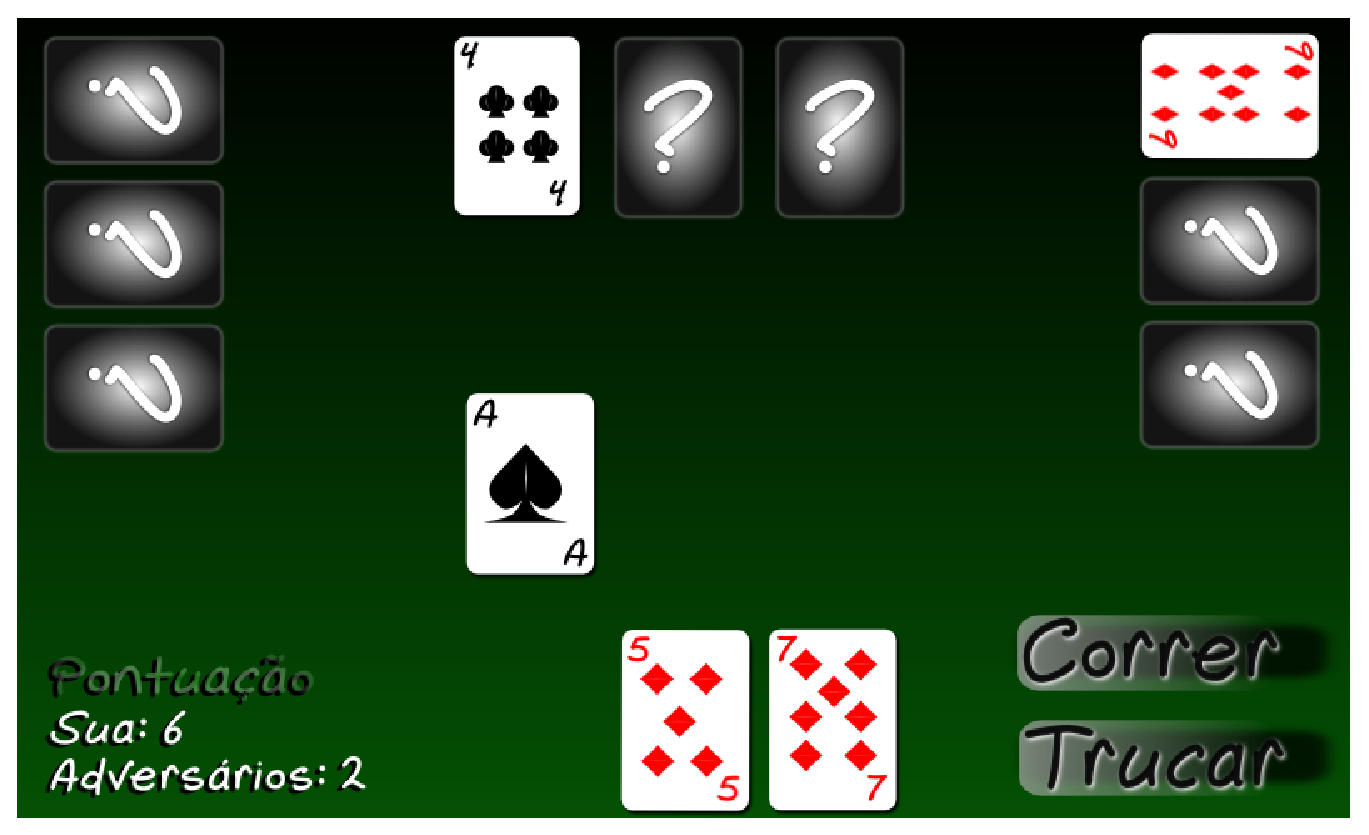
\includegraphics[scale=0.35]{images/screen-in_game-n800.eps}
    \caption{Esquema do funcionamento do BRisa Game Server(BRiGaS).}
    \label{fig:avschema_new}
\vspace{-5mm}
\end{figure}
\vspace{3mm}
\normalsize

>>>>>>> MERGE-SOURCE
\section{Trabalhos Futuros}
Com o desenvolvimento do trabalho algumas necessidades e possibilidades de aperfeiçoamento forma observados, inclusive sobre limitações do próprio padrão UPnP. Primeiramente, a criação de uma extensão para o protocolo UPnP, pois devido às limitações do mesmo com relação ao envio de eventos multicast vários pacotes desnecessários são enviados pela rede, sabe-se que é dessa forma que os Control Points recebem a notificação das mudanças de variáveis de estado. Ainda não há uma forma de envio de eventos unicast, portanto a nova extensão deve especificar uma forma de envio de eventos unicast, tendo em vista que ainda não há uma forma unicast de prover essa comunicação, ou seja fazer a comunicação entre um dispositivo e um control point específico.

Em relação ao próprio BRiGaD, há a necessitade da especificação de um esquema de segurança e criptografia no trânsito de algumas mensagem enviadas e recebidas pelo Game Server para dificultar o 'crackeamento' dos jogos. Outro trabalho é a identificação única dos jogadores, para criar perfis no servidor, estabelecendo ranking e reputação. Uma solução é utilizar a extensão UPnP-UP[!!!!??!?!!] para prover essa funcionalidade.

Com a identificação do usuário através do UPnP-UP pode-se também criar um sistema de personalização do jogo, onde o jogador pode mudar suas configurações no servidor, e esta personalização pode ser carregada para qualquer servidor de jogos que o jogador se conectar. Ainda com o UPnP-UP pode ser feito um esquema de recomendação de jogos, oponentes e parceiros, devido ao armazenamento das preferências e histórico do usuário. Recomendar oponentes também é significativo, pois  aumenta a competitividade dentro do servidor, os jogadores que estão no mesmo nível de habilidade poderão jogar uns contra os outros. Os parceiros em jogos que mais obtiveram vitórias podem ser recomendados para jogarem juntos novamente, já que teoricamente eles possuem um introsamento maior.

\section{Conclusão}
Neste artigo foi demonstrado a criação de uma especificação para servidores de jogos utilizando o padrão UPnP. Com a especificação definimos a um novo dispositivo (UPnP device), o Game Server, e seus serviços, o Game Manager. Para provar os conceitos dessa especificação, a ferramenta foi implementada utilizando o framework BRisa para o padrão UPnP.  Além disso, foi apresentada a implementação de um jogo de Truco citada como estudo de caso.

%\bibliographystyle{sbgames}
%\bibliography{template}
\end{document}
